\documentclass[titlepage]{article}

\usepackage[letterpaper,margin=1in,footskip=0.25in]{geometry}
\usepackage[hidelinks]{hyperref}
\usepackage{fancyhdr}
\usepackage{csquotes}
\usepackage{amsmath}
\usepackage{tikz}
\usepackage[list=true]{subcaption}
\usepackage{graphicx}
\usepackage{amssymb}

\MakeOuterQuote{"}

\numberwithin{figure}{section}

\usetikzlibrary{knots,decorations.markings}

\newcommand{\dq}[2]{``#1" (#2).}

\renewcommand{\labelitemiii}{\scriptsize$\blacksquare$}

\title{{\Huge\emph{The Knot Book}}\\[5pt]\textcolor{gray!60!black}{Notes}\vspace{-0.5em}}
\author{Steven Labalme}
\date{\today}

\begin{document}




\pagenumbering{gobble}
\maketitle



\pagenumbering{roman}
\tableofcontents
\listoffigures
\listoftables
\newpage



\pagenumbering{arabic}
\pagestyle{fancy}
\fancyhf{}
\rfoot{Labalme \thepage}
\renewcommand{\headrulewidth}{0pt}
\section{Introduction}\label{sse:intro}
\subsection{Introduction}
\begin{itemize}
    \item \textbf{Knot}: \dq{A knotted loop of string, except that we think of the string as having no thickness, its cross-section being a single point}{2}
    \item Do not distinguish between a `nice, even' knot and one that has been deformed through space.
    \item \textbf{Unknot}: \dq{The simplest knot of all\dots the unknoted circle}{2} \emph{Also known as} \textbf{trivial knot}. See Figure \ref{fig:circletrefoila}.
    \item \textbf{Trefoil knot}: \dq{The next simplest knot}{2} See Figure \ref{fig:circletrefoilb}.
    \begin{figure}[h!]
        \centering
        \begin{subfigure}{0.2\linewidth}
            \centering
            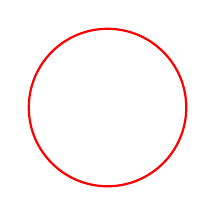
\begin{tikzpicture}
                \draw[red,thick] (0,0) circle (1cm);
            \end{tikzpicture}
            \caption{Trivial knot.}
            \label{fig:circletrefoila}
        \end{subfigure}
        \begin{subfigure}{0.2\linewidth}
            \centering
            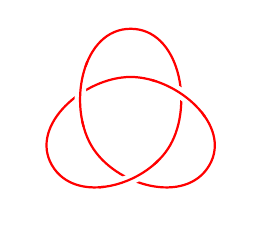
\begin{tikzpicture}
                \begin{knot}[
                    consider self intersections,
                    clip width=5
                ]
                    % could be defined with a combination of polar coordinates and foreach...
                    \strand[red,thick] (1,{3^0.5})
                        to [out=0,in=60] (1.5,0.25)
                        to [out=240,in=-60] (0,0)
                        to [out=120,in=180] (1,1.12)
                        to [out=0,in=60] (2,0)
                        to [out=240,in=-60] (0.5,0.25)
                        to [out=120,in=180] cycle
                    ;
                    \flipcrossings{1,3}
                \end{knot}
            \end{tikzpicture}
            \caption{Trefoil knot.}
            \label{fig:circletrefoilb}
        \end{subfigure}
        \caption{Projections of the two simplest knots.}
        \label{fig:circletrefoil}
    \end{figure}
    \item \textbf{Projection}: A picture of a knot, such as those in Figure \ref{fig:circletrefoil}.
    \begin{itemize}
        \item The same knots can have multiple projections (as they are deformed in space).
    \end{itemize}
    \item \textbf{Crossings}: The places in a projection where a knot crosses itself.
    \begin{itemize}
        \item The trefoil knot in Figure \ref{fig:circletrefoilb} is a \underline{three-crossing knot} because it crosses itself 3 times.
        \item Any one-crossing knot is trivial.
        \item \emph{Exercise 1.2}: Any two-crossing knot must be trivial because the simplest nontrivial knot is the trefoil knot, which has three crossings.
    \end{itemize}
    \item Atoms were originally thought to be tangles (knots) in the ether of the universe, but when chemists moved on, mathematicians took up knot theory. In the 1980s, biochemists began to see applications of knot theory in their research (see Section \ref{sse:biochemphys}).
    \item \textbf{Topology}: \dq{The study of the properties of geometric objects that are preserved under deformations}{6}
    \begin{itemize}
        \item Knot theory is a subfield of topology (see Section \ref{sse:topology}).
    \end{itemize}
    \begin{figure}[h!]
        \centering
        \includegraphics[width=0.7\linewidth]{Blender/CubeSphere.png}
        \caption{Deformation of a cube into a sphere.}
        \label{fig:cubesphere}
    \end{figure}
    \item Any knot can have a projection with as many crossings as desired.
    \item \textbf{Alternating knot}: \dq{A knot with a projection that has crossings that alternate between over and under as one travels around the knot in a fixed direction}{7}
    \begin{itemize}
        \item The trefoil is such a knot.
    \end{itemize}
    \item \emph{Exercise 1.7*}: By changing some of the crossings from over to under or vice versa, any projection of a knot can be made into a projection of the unknot$^[$\footnote{How can I \emph{show} something? How can I do these proofs? What kind of logic solves one of these?}$^]$. See Figure \ref{fig:knottotrivial}.
    \begin{figure}[h!]
        \centering
        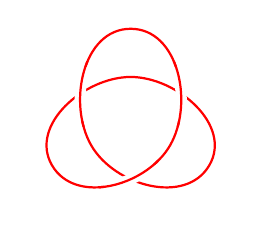
\begin{tikzpicture}
            \begin{knot}[
                consider self intersections,
                clip width=5
            ]
                \strand[red,thick] (1,{3^0.5})
                    to [out=0,in=60] (1.5,0.25)
                    to [out=240,in=-60] (0,0)
                    to [out=120,in=180] (1,1.12)
                    to [out=0,in=60] (2,0)
                    to [out=240,in=-60] (0.5,0.25)
                    to [out=120,in=180] cycle
                ;
                \flipcrossings{3}
            \end{knot}
        \end{tikzpicture}
        \caption{A projection of the unknot evoking the trefoil knot.}
        \label{fig:knottotrivial}
    \end{figure}
\end{itemize}


\subsection{Composition of Knots}
\begin{itemize}
    \item \textbf{Composition} (of two knots): \dq{A new knot obtained by removing a small arc from two knot projections and then connecting the four endpoints by two new arcs}{7}
    \begin{itemize}
        \item If two knots are designated $J$ and $K$, then their composition is denoted $J\#K$.
        \item Do not overlap the projections and choose two arcs that are on the outside to avoid new crossings.
        \item Make sure that the new arcs do not cross any of the the original knot projections or each other.
    \end{itemize}
    \item \textbf{Composite knot}: A knot that \dq{can be expressed as the composition of two knots, neither of which is the trivial knot}{8}
    \begin{itemize}
        \item This definition is analogous to composite integers, where an integer is \underline{composite} if it is the product of positive integers, neither of which is $1$.
        \item Similarly, if we compose any knot with the unknot, we get the same knot back.
    \end{itemize}
    \item \textbf{Factor knots}: \dq{The knots that make up the composite knot}{8}
    \item \textbf{Prime knot}: \dq{A knot [that] is not the composition of any two nontrivial knots}{9}
    \item The unknot, trefoil knot, and figure-eight knots are all prime (see Section \ref{sss:GenusSeifert}).
    \begin{itemize}
        \item The unknot is not composite for the same reason that 1 is not the product of two integers greater than 1.
    \end{itemize}
    \begin{figure}[h!]
        \centering
        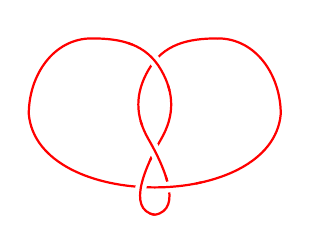
\begin{tikzpicture}[scale=0.8]
            \begin{knot}[
                clip width=5
            ]
                % Use looseness=# key to stretch out lengths!
                \strand[red,thick]       (0,0)
                    to [out=-85,in=-95]  (4,0)
                    to [out=90,in=0]     (3,1.2)
                ;
                \strand[red,thick]       (3,1.2)
                    to [out=180,in=60]   (1.9,0.7)
                    to [out=-120,in=120] (1.9,-0.4)
                    to [out=-60,in=10]   (2,-1.6)
                ;
                \strand[red,thick]       (2,-1.6)
                    to [out=170,in=-120] (2.1,-0.4)
                    to [out=60,in=-60]   (2.1,0.7)
                    to [out=120,in=0]    (1,1.2)
                    to [out=180,in=90]   (0,0)
                ;
                \flipcrossings{2,3}
            \end{knot}
        \end{tikzpicture}
        \caption{The figure-eight knot.}
        \label{fig:figure8knot}
    \end{figure}
    \item Similar to integers, \dq{a composite knot factors into a unique set of prime knots}{10}
    \newpage
    \item \emph{Exercise 1.8}: Using the appendix table, identify the factor knots that make up the composite knot in Figure \ref{fig:compos1}.
    \begin{figure}[h!]
        \centering
        \includegraphics[width=0.15\linewidth]{Blender/compos1.png}
        \caption{The composite knot.}
        \label{fig:compos1}
    \end{figure}
    \begin{itemize}
        \item \textsc{Figure out when knot cord arrives.}
    \end{itemize}
    \item \emph{Exercise 1.9}: Show that the knot in Figure \ref{fig:compos2a} is composite.
    \begin{figure}[h!]
        \centering
        \begin{subfigure}[b]{0.3\textwidth}
            \centering
            \includegraphics[width=0.5\textwidth]{Blender/compos2.png}
            \caption{The composite knot.}
            \label{fig:compos2a}
        \end{subfigure}
        \begin{subfigure}[b]{0.3\textwidth}
            \centering
            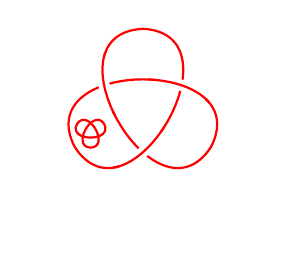
\begin{tikzpicture}
                \begin{knot}[
                    clip width=5,
                    consider self intersections
                ]
                    % Why don't polar coordinates mesh with figures?
                    \strand[red,thick] (90:1)
                        \foreach \x in {1,2,3} {
                            to [bend left=117,looseness=1.9] ({90+120*\x}:1)
                        }
                    ;
                    \flipcrossings{1,3}
                \end{knot}
                \begin{knot}[
                    clip width=5,
                    consider self intersections,
                    rotate=60,
                    scale=0.2,
                    xshift=-3cm,yshift=2.1cm
                ]
                    \strand[red,thick] (90:1)
                        \foreach \x in {1,2,3} {
                            to [bend left=117,looseness=1.9] ({90+120*\x}:1)
                        }
                    ;
                    \flipcrossings{1,3}
                \end{knot}
            \end{tikzpicture}
            \vspace{-0.8cm}
            \caption{Factors.}
            \label{fig:compos2b}
        \end{subfigure}
        \caption{Factorization of a `double trefoil.'}
        \label{fig:compos2}
    \end{figure}
    \item There is more than one way to take the composition of two knots (by removing different arcs).
    \begin{itemize}
        \item This is not analogous to multiplication --- a break in the pattern.
    \end{itemize}
    \item \textbf{Orientation}: A direction to travel around the knot. Denoted by placing \dq{coherently directed arrows along the projection of the knot in the direction of our choice}{10} A knot with such arrows is \textbf{oriented}.
    \begin{itemize}
        \item All compositions $J\#K$ where the orientations of $J$ and $K$ \underline{do} match up will yield the same composite knot.
        \begin{itemize}
            \item $J$ can be `slid around' $J\#K$ until it reaches the second position where the composition was taken.
        \end{itemize}
        \item All compositions $J\#K$ where the orientations of $J$ and $K$ \underline{do not} match up will yield the same composite knot.
        \item These two compositions can be distinct.
    \end{itemize}
    \begin{figure}[h!]
        \centering
        \begin{tikzpicture}
            \begin{knot}[
                clip width=5,
                consider self intersections
            ]
                \strand[red,thick,
                decoration={markings,
                mark=at position 0.2 with {\arrow{>}}},
                postaction={decorate}] (90:1)
                    \foreach \x in {1,2,3} {
                        to [bend left=117,looseness=1.9] ({90+120*\x}:1)
                    }
                ;
                \flipcrossings{1,3}
            \end{knot}
        \end{tikzpicture}
        \vspace{-0.8cm}
        \caption{Orientation notation.}
        \label{fig:orientnotation}
    \end{figure}
    \item \textbf{Invertible}: A knot that can be deformed back to itself so that an orientation on it is sent to the opposite orientation.
    \begin{itemize}
        \item \dq{In the case that one of the two knots is invertible, say $J$, we can always deform the composite knot so that the orientation on $K$ is reversed, and hence so that the orientations of $J$ and $K$ always match. Therefore, there is only one composite knot that we can construct from the two knots}{11}
    \end{itemize}
    \item To determine the possible compositions of knots, it is necessary to know which knots are invertible, but no general technique has yet been discovered.
\end{itemize}


\subsection{Reidemeister Moves}
\begin{itemize}
    \item \textbf{Ambient isotropy}: \dq{The movement of the string through three-dimensional space without letting it pass through itself}{12}
    \item \textbf{Planar isotropy}: A deformation of \dq{the projection plane as if it were made of ruber with the projection drawn upon it}{12}
    \begin{itemize}
        \item Stretching, squeezing, rotating, bending single arcs, etc.
    \end{itemize}
    \item \textbf{Reidemeister move}: \dq{One of three ways to change a projection of the knot that \emph{will} change the relation between the crossings}{13}
    \item \textbf{First Reidemeister move}: \dq{Put in or take out a twist in the knot}{13} See Figure \ref{fig:reidema}. \emph{Also known as} \textbf{type I Reidemeister move}.
    \item \textbf{Second Reidemeister move}: \dq{Either add two crossings or remove two crossings}{13} See Figure \ref{fig:reidemb}. \emph{Also known as} \textbf{type II Reidemeister move}.
    \item \textbf{Third Reidemeister move}: \dq{Slide a strand of the knot from one side of a crossing to the other side of the crossing}{13} See Figure \ref{fig:reidemc}. \emph{Also known as} \textbf{type III Reidemeister move}.
    \begin{itemize}
        \item Note that the crossings in Figure \ref{fig:reidem} can be reversed and the move will still be classified under the same category.
    \end{itemize}
    \begin{figure}[h!]
        \centering
        \begin{subfigure}[b]{0.3\linewidth}
            \centering
            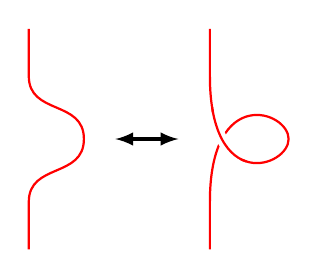
\begin{tikzpicture}
                \draw[red,thick,xshift=-1.5cm] (0,0.4) -- (0,1) .. controls (0,1.5) and (0.7,1.3) .. (0.7,1.8) .. controls (0.7,2.3) and (0,2.1) .. (0,2.6) -- (0,3.2);
                \draw[very thick,latex-latex] (-0.4,1.8) -- (0.4,1.8);
                \begin{knot}[
                    xshift=0.8cm,
                    consider self intersections=no splits,
                    clip width=5,
                    flip crossing=1
                ]
                    \strand[red,thick] (0,0.4) -- (0,1) to [out=90,in=90,out looseness=3,in looseness=0.7] (1,1.8) to [out=-90,in=-90,in looseness=3,out looseness=0.7] (0,2.6) -- (0,3.2);
                \end{knot}
            \end{tikzpicture}
            \caption{Type I Reidemeister move.}
            \label{fig:reidema}
        \end{subfigure}
        \begin{subfigure}[b]{0.3\linewidth}
            \centering
            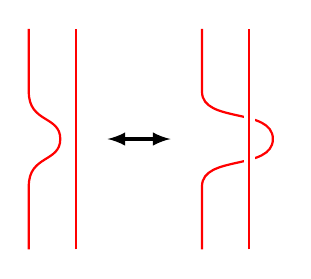
\begin{tikzpicture}
                \draw[red,thick,xshift=-1.4cm] (0,0.4) -- (0,1.2) .. controls (0,1.6) and (0.4,1.5) .. (0.4,1.8) .. controls (0.4,2.1) and (0,2) .. (0,2.4) -- (0,3.2);
                \draw[red,thick,xshift=-1.4cm] (0.6,0.4) -- (0.6,3.2);
                \draw[very thick,latex-latex] (-0.4,1.8) -- (0.4,1.8);
                \begin{knot}[
                    xshift=0.8cm,
                    clip width=5
                ]
                    \strand[red,thick] (0,0.4) -- (0,1.2) .. controls (0,1.6) and (0.9,1.4) .. (0.9,1.8) .. controls (0.9,2.2) and (0,2) .. (0,2.4) -- (0,3.2);
                    \strand[red,thick] (0.6,0.4) -- (0.6,3.2);
                    \flipcrossings{1,2}
                \end{knot}
            \end{tikzpicture}
            \caption{Type II Reidemeister move.}
            \label{fig:reidemb}
        \end{subfigure}\\
        \vspace{1em}
        \begin{subfigure}[b]{0.6\linewidth}
            \centering
            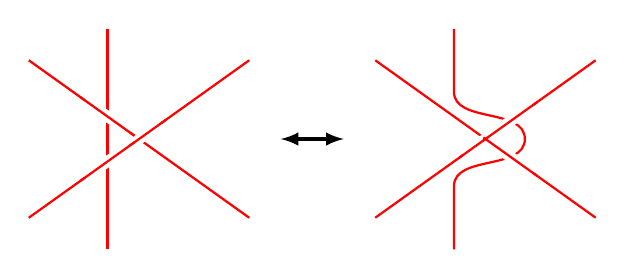
\begin{tikzpicture}
                \begin{knot}[
                    xshift=-2.2cm,
                    clip width=5
                ]
                    \strand[red,thick] (-1.4,0.8) -- (1.4,2.8);
                    \strand[red,thick] (-1.4,2.8) -- (1.4,0.8);
                    \strand[red,thick] (-0.4,0.4) -- (-0.4,3.2);
                \end{knot}
                \draw[very thick,latex-latex] (-0.4,1.8) -- (0.4,1.8);
                \begin{knot}[
                    xshift=2.2cm,
                    clip width=5
                ]
                    \strand[red,thick] (-1.4,0.8) -- (1.4,2.8);
                    \strand[red,thick] (-1.4,2.8) -- (1.4,0.8);
                    \strand[red,thick] (-0.4,0.4) -- (-0.4,1.2) .. controls (-0.4,1.6) and (0.5,1.4) .. (0.5,1.8) .. controls (0.5,2.2) and (-0.4,2) .. (-0.4,2.4) -- (-0.4,3.2);
                \end{knot}
            \end{tikzpicture}
            \caption{Type III Reidemeister move.}
            \label{fig:reidemc}
        \end{subfigure}
        \caption{Reidemeister moves.}
        \label{fig:reidem}
    \end{figure}
    \item All Reidemeister moves are ambient isotropies.
    \item \dq{If we have two distinct projections of the same knot, we can get from the one projection to the other by a series of Reidemeister moves and planar isotropies}{14}
    \item \textbf{Amphicheiral}: A knot that \dq{is equivalent to its mirror image, that is, the knot obtained by changing every crossing\dots to the opposite crossing}{14-15} \emph{Also known as} \textbf{achiral} \emph{by chemists.}
    \begin{itemize}
        \item A knot and its mirror image are distinct unless the knot is amphicheiral.
        \item See Section \ref{sse:biochemphys} for more on amphicheirality.
    \end{itemize}
    \item \emph{Exercise 1.10}: Show that the two projections in Figure \ref{fig:ex1-10} represent the same knot by finding a series of Reidemeister moves from one to the other.
    \begin{figure}[h!]
        \centering
        \begin{subfigure}[b]{0.2\linewidth}
            \centering
            \includegraphics[width=0.6\linewidth]{Blender/ex1-10a.png}
            \caption{Initial projection.}
            \label{fig:ex1-10a}
        \end{subfigure}
        \begin{subfigure}[b]{0.2\linewidth}
            \centering
            \includegraphics[width=0.4\linewidth]{Blender/ex1-10b.png}
            \vspace{4mm}
            \caption{Final projection.}
            \label{fig:ex1-10b}
        \end{subfigure}
        \caption{Finding Reidemeister moves.}
        \label{fig:ex1-10}
    \end{figure}
    \begin{figure}[h!]
        \centering
        \includegraphics[width=0.8\linewidth]{Blender/ex1-10-2.png}
        \caption{Solution to \emph{Exercise 1.10}.}
        \label{fig:ex1-10-2}
    \end{figure}
    \item \emph{Exercise 1.11*}: Find a sequence of Reidemeister moves to untangle the unknot shown in Figure \ref{fig:ex1-11}.
    \begin{figure}[h!]
        \centering
        \includegraphics[width=0.17\linewidth]{Blender/ex1-11.png}
        \caption{Unknot to be untangled.}
        \label{fig:ex1-11}
    \end{figure}
    \begin{figure}[h!]
        \centering
        \includegraphics[width=0.8\linewidth]{Blender/ex1-11-2.png}
        \caption{Solution to \emph{Exercise 1.11*}.}
        \label{fig:ex1-11-2}
    \end{figure}
    \item The bounds on the increase in crossings generated by Reidemeister moves from one projection to another are unknown.
\end{itemize}


\subsection{Links}
\begin{itemize}
    \item \textbf{Link}: A set of knotted loops all tangled up together.
    \item \dq{Two links are considered to be the same if we can deform the one link to the other link without ever having any one of the loops intersect itself or any of the other loops in the process}{17}
    \begin{figure}[h!]
        \centering
        \begin{subfigure}[b]{0.2\linewidth}
            \centering
            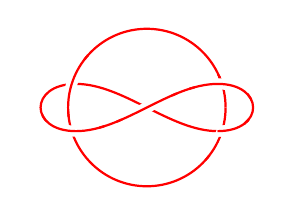
\begin{tikzpicture}
                \begin{knot}[
                    clip width=5,
                    ignore endpoint intersections=false,
                    consider self intersections=true
                ]
                    \strand[red,thick] circle (1cm);
                    \strand[red,thick] plot[smooth cycle,tension=1.2] coordinates{
                        (-0.9,0.3) (0.9,-0.3) (0.9,0.3) (-0.9,-0.3)
                    };
                    \flipcrossings{3,5}
                \end{knot}
            \end{tikzpicture}
            \caption{Whitehead link.}
            \label{fig:WhiteheadBorromeana}
        \end{subfigure}
        \begin{subfigure}[b]{0.2\linewidth}
            \centering
            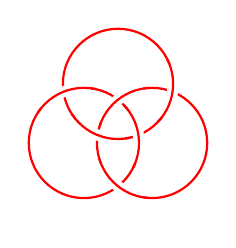
\begin{tikzpicture}
                \begin{knot}[
                    clip width=5
                ]
                    \strand[red,thick] (90:0.5)  circle (0.7cm);
                    \strand[red,thick] (210:0.5) circle (0.7cm);
                    \strand[red,thick] (330:0.5) circle (0.7cm);
                    \flipcrossings{1,2,5,6}
                \end{knot}
            \end{tikzpicture}
            \caption{Borromean rings.}
            \label{fig:WhiteheadBorromeanb}
        \end{subfigure}
        \caption{Projections of two simple links.}
        \label{fig:WhiteheadBorromean}
    \end{figure}
\end{itemize}





\end{document}



% \subsection{Tricolorability}
% \begin{itemize}
%     \item \dq{hi}{\#\#}
% \end{itemize}


% \subsection{Knots and Sticks}
% \begin{itemize}
%     \item \dq{hi}{\#\#}
% \end{itemize}